%----------------------------------------------------------------------------------------
%	PACKAGES AND DOCUMENT CONFIGURATIONS
%----------------------------------------------------------------------------------------

\documentclass{article}

\usepackage{graphicx} % Required for the inclusion of images
\usepackage{natbib} % Required to change bibliography style to APA
\usepackage{amsmath} % Required for some math elements 
\usepackage{placeins}
\usepackage[font=small,labelsep=space]{caption}
\captionsetup{%
  figurename=Fig.,
  tablename=Table
}
\setcitestyle{square}
\setlength\parindent{0pt} % Removes all indentation from paragraphs

\renewcommand{\eqref}[1]{\textup{{\normalfont(\ref{#1}}\normalfont)}}

\renewcommand{\labelenumi}{\alph{enumi}.} % Make numbering in the enumerate environment by letter rather than number (e.g. section 6)

%\usepackage{times} % Uncomment to use the Times New Roman font

\textheight=8.5in
\topmargin=-0.5in

%----------------------------------------------------------------------------------------
%	DOCUMENT INFORMATION
%----------------------------------------------------------------------------------------

\title{Homework 1} % Title

\author{Kenneth \textsc{Chaney}} % Author name

\date{\today} % Date for the report

\begin{document}

\maketitle % Insert the title, author and date

\begin{center}
\begin{tabular}{l r}
Date Performed: & November \(13^{th}\), 2014 \\ % Date the experiment was performed
Instructor: & Professor Dandekar \\ % Instructor/supervisor
Class: & ECET-512
\end{tabular}
\end{center}

% If you wish to include an abstract, uncomment the lines below
\begin{abstract}
The goal of this homework is to simulate a single user traveling through a cellular network while using new path loss equations in Part A. The co-channel interference (CCI) is also observed within this cellular network in Part B. Finally the signal to interference ratio (SIR) is analyzed in Part C.

\end{abstract}

\pagebreak
%----------------------------------------------------------------------------------------
%	SECTION 1
%----------------------------------------------------------------------------------------

\section{Part A}\label{partA}

To generate results for this section run the demoA.m file. The animation generated shows the mobile user traveling across a cell boundry simulating a handoff situation. There are several accompanying plots shown in figure \ref{parta}.\\

The path loss model used is shown in equation \ref{pathloss}. Since the shadowing is random the handoff will occur at different times throughout the process during each run. There is also a no shadowing signal that is tracked to show where the ideal handoff would occur. Due to the random nature of shadowing, it imposed several constraints into the design. First, we don't want to throw a user back to the original cell immediately after handoff has occured. Second, we don't want to complete the handoff until the signal from the second base station rises above \( P_{r,H0} \). Third, we need to filter out the noise in the signal. This drove the design of a simple state-machine system that only changed state based on the analysis of the filtered signal. The state machine kept track of what state the user was in--connected to BS1, in handoff, connected to BS2--this allowed for there to be distinct conditions for each stage. These conditions were found using the mean of the previous six values--this is simplistic but gets the job done for our case. \\

\begin{equation}\label{pathloss}
P_r(d)=E\begin{bmatrix}P_r(d_0)\end{bmatrix}-10\beta log_{10}\dfrac{d}{d_0}+\epsilon
\end{equation}

\begin{figure}[h]
\centerline{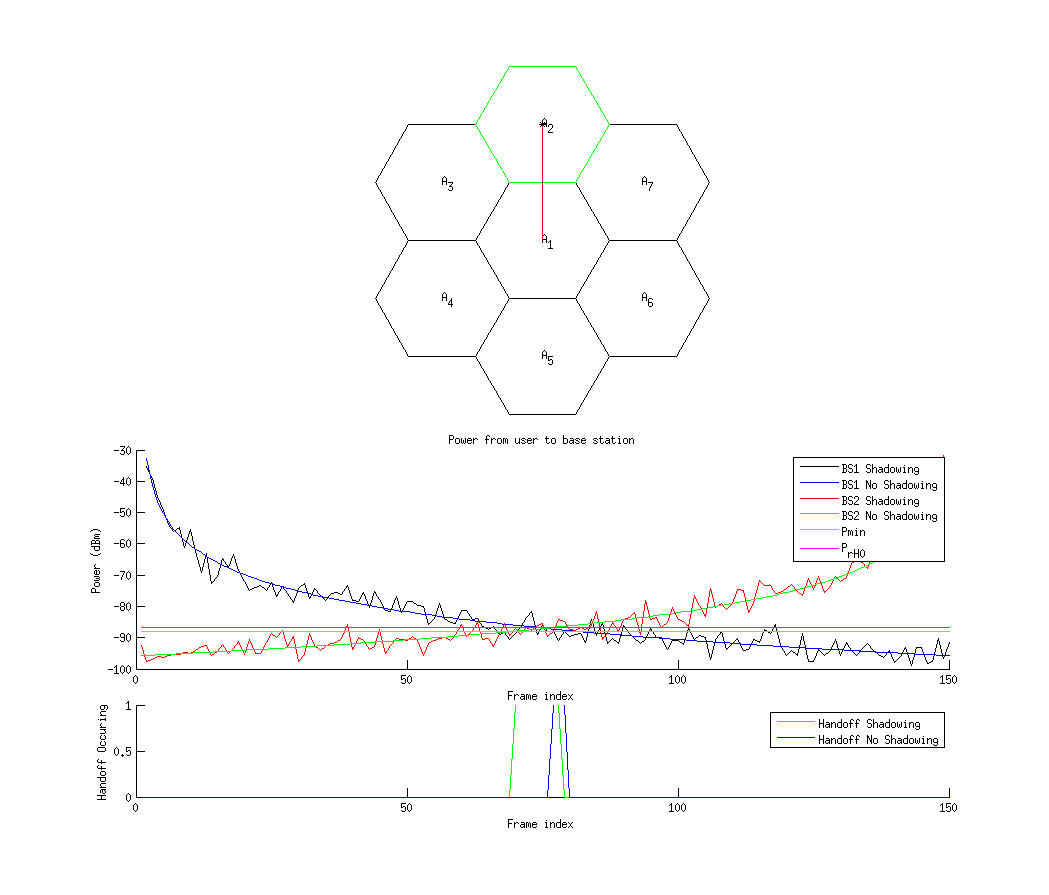
\includegraphics[width=5in]{doc/partA.png}}
\caption{Mobile user handoff simulation. Top plot is the user traveling through the space. Second is the user's signal realative to base stations. Bottom is whether or not a handoff is occuring for the shadowing or no shadowing data.}
\label{parta}
\end{figure}

\clearpage

\section{Part B}\label{partB}

To generate results for this section run the demoB.m file. A similar animation to Part A will show up--a sample figure is shown in figure \ref{partb}. \\

The lower graph displays a legend to correspond the line with the base station, however for values of n>1 this looks poor. This demonstration shows the need for high efficiency systems in cases where multiple users culminate in any singular location. This can be seen in the n=1 case where towards the middle of the simulation most users are in the center--in this case the outter users may be pushed to a neighboring base station. The trunking efficiency is needed within a cellular network to be able to deal with unusual cases where users density differs. There won't be a realistic system where user density is constant throughout time--so a dynamic system is also needed to ensure maximum quality.\\

The call blocking can be simulated using a markov chain for each base station to keep track of system resources over time to allow or deny a call based on the current state. Each user can attempt to initiate a call to their current base station during random time increments. The last important consideration is the fact that users will have to switch cells while moving--so a system will have to be put in place that keeps track of a user leaving one system and entering another (this can be simple--disconnect and connect "instantaneously"--or complex--special channels for the handoff to occur to ensure the call won't be dropped).\\

\begin{figure}[h]
\centerline{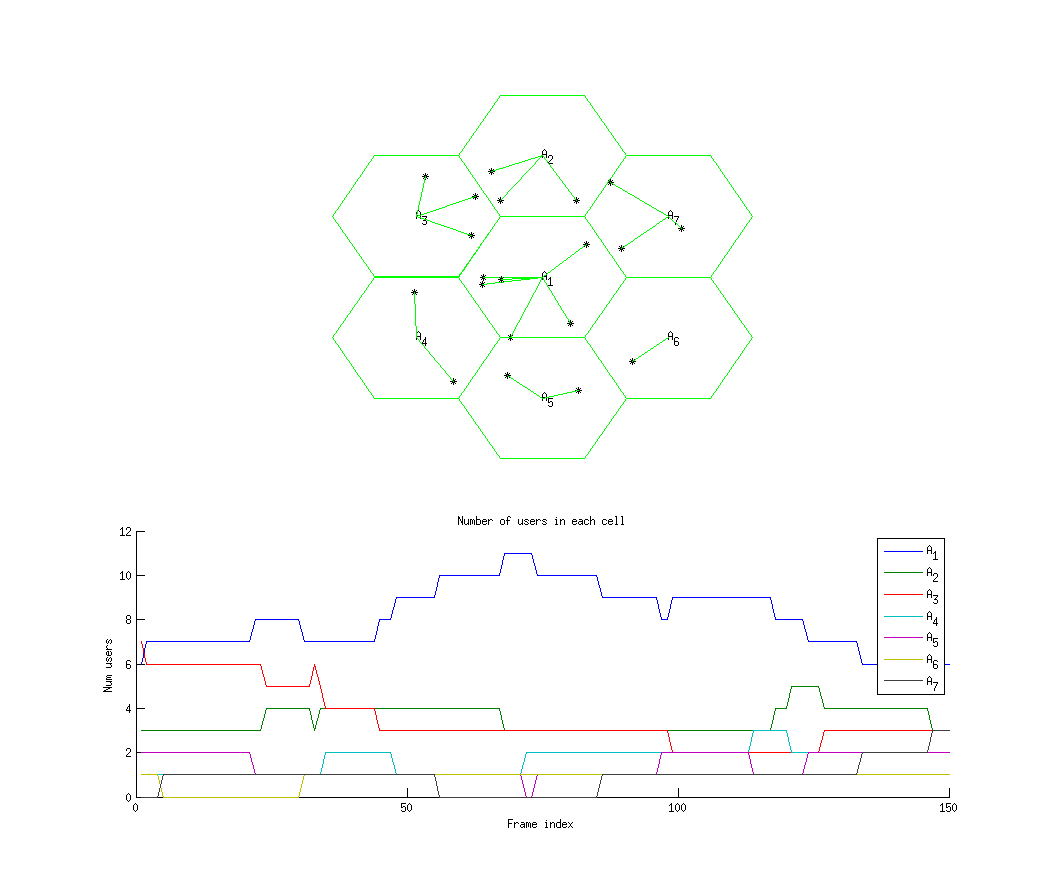
\includegraphics[width=5in]{doc/partB.png}}
\caption{Multiple users within cellular network. Top plot is each user moving along their trajectory (green cells are being used). Bottom plot is the connected users to each cell.}
\label{partb}
\end{figure}

\end{document}
